\documentclass[letterpaper, 12pt]{article}

%%%%%%%%%%%%%%%%%%%    PACKAGES    %%%%%%%%%%%%%%%%%%%
%% font
\usepackage{fontspec}

%% languages
\usepackage{polyglossia}
	\setdefaultlanguage[variant=british]{english}

%% marges, space...
\usepackage[top=2.5cm, bottom=2.5cm, left=2.5cm, right=2.5cm]{geometry}

%% Graphics
\usepackage[luatex]{graphicx}

%%%%%%%%%%%%%%%%%%%%%%%%%%%%%%%%%%%%%%%%%%%%%%%%%%%%%%

\begin{document}
\section{MCMCs trace plots and histograms}
\begin{figure}[h]
	\centering
	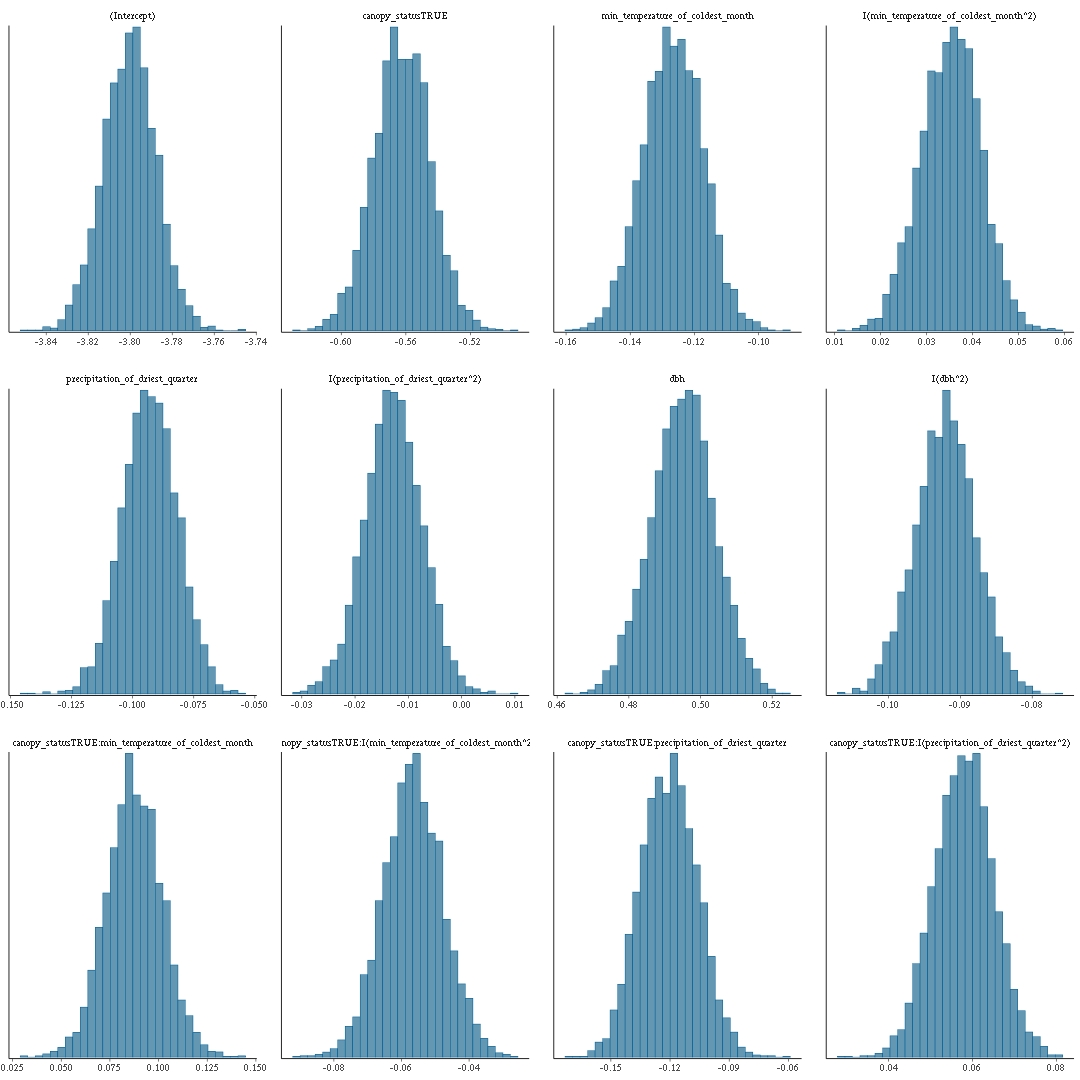
\includegraphics[scale=0.4]{./18032-ABI-BAL_hist}
	\caption{\textit{Abies balsamea}}
\end{figure}

\begin{figure}
	\centering
	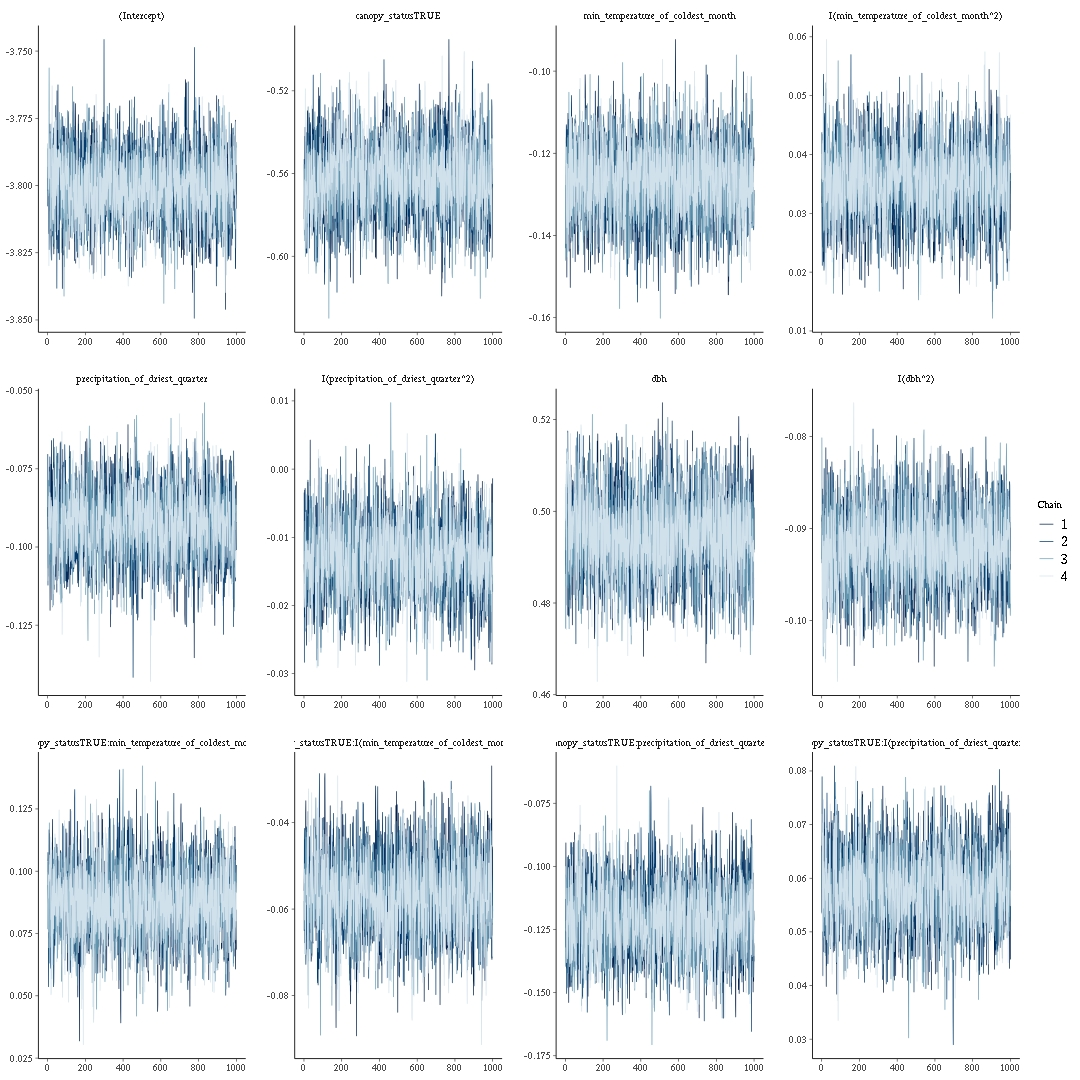
\includegraphics[scale=0.4]{./18032-ABI-BAL_traces}
	\caption{\textit{Abies balsamea}}
\end{figure}

\begin{figure}
	\centering
	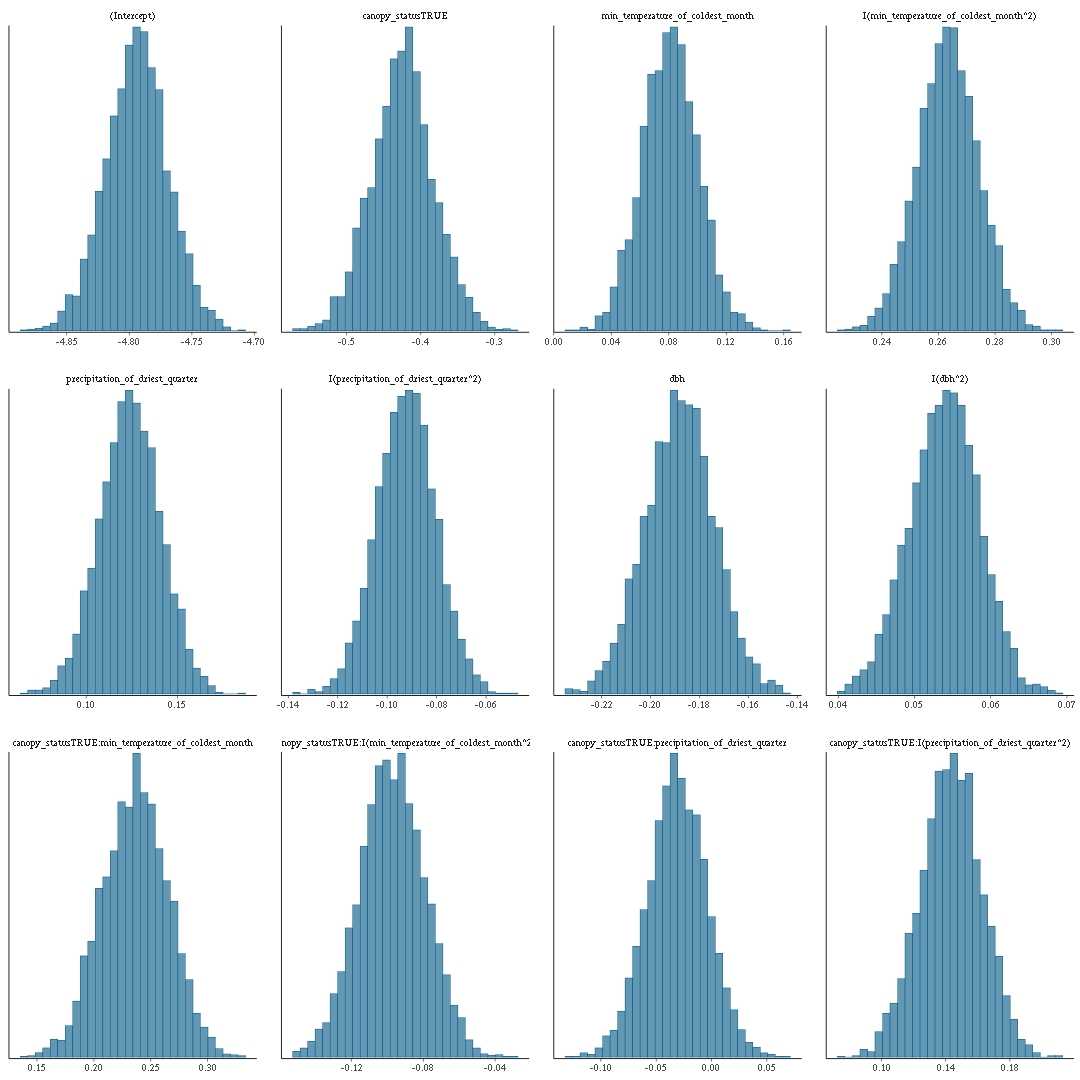
\includegraphics[scale=0.4]{./28728-ACE-RUB_hist}
	\caption{\textit{Acer rubrum}}
\end{figure}

\begin{figure}
	\centering
	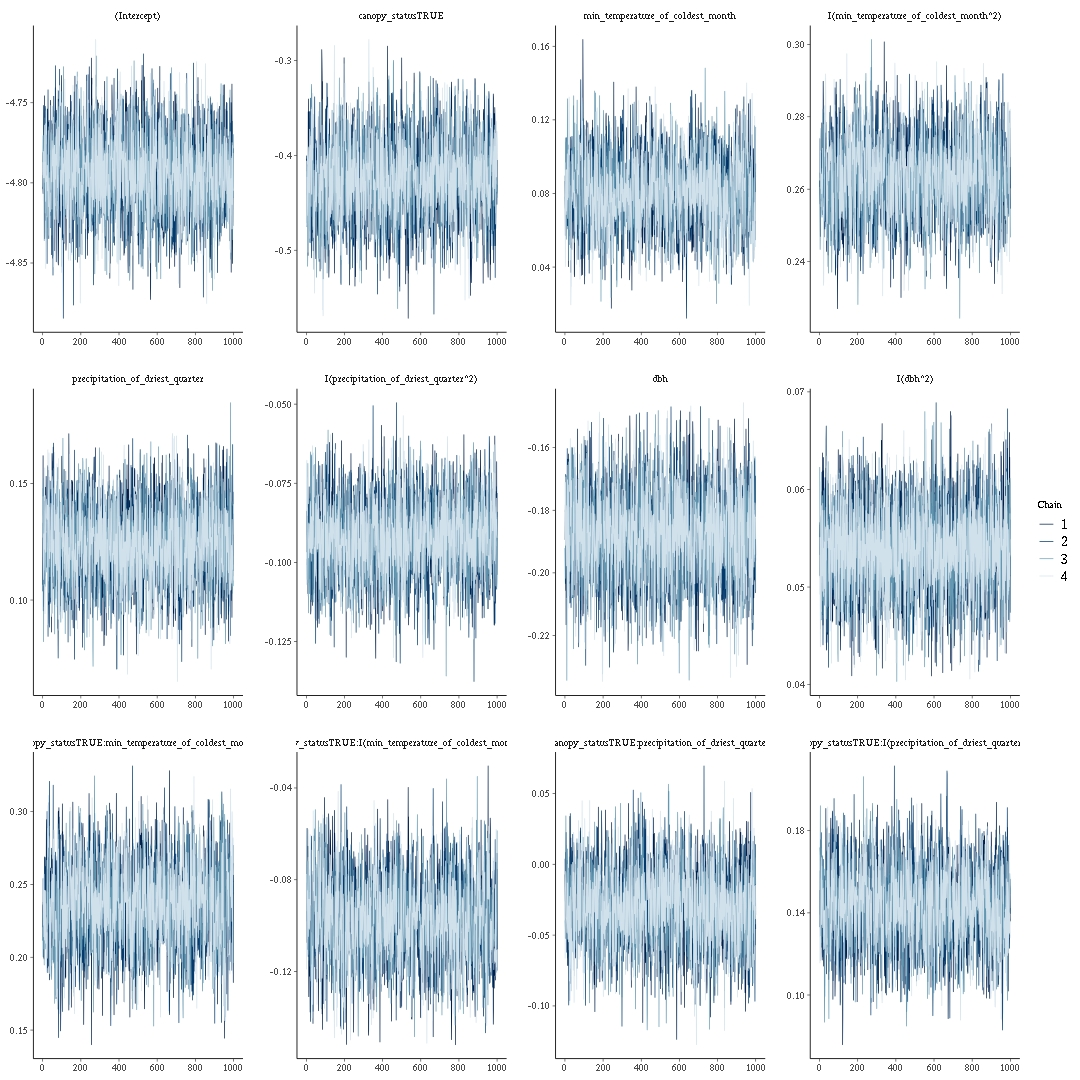
\includegraphics[scale=0.4]{./28728-ACE-RUB_traces}
	\caption{\textit{Acer rubrum}}
\end{figure}

\begin{figure}
	\centering
	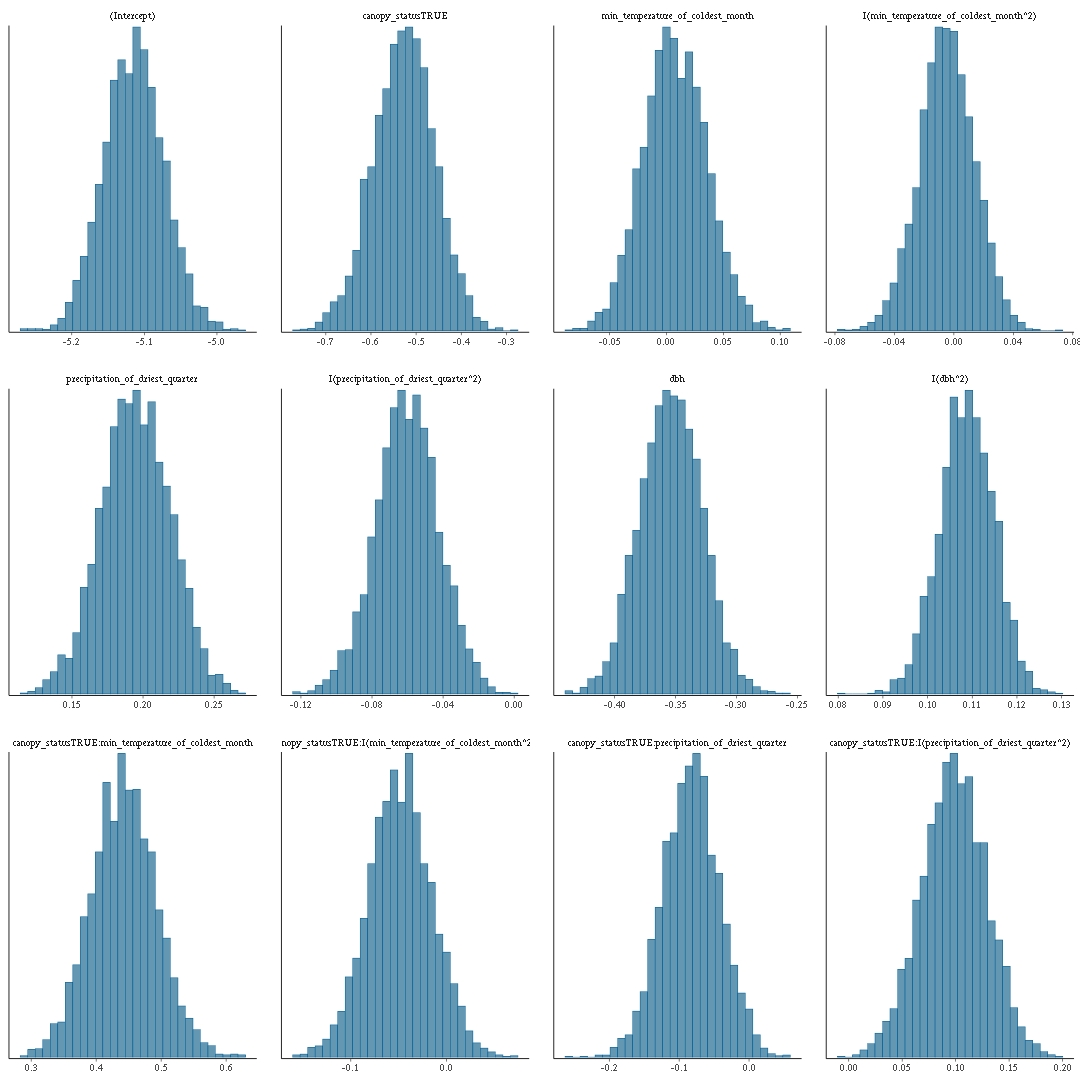
\includegraphics[scale=0.4]{./28731-ACE-SAC_hist}
	\caption{\textit{Acer saccharum}}
\end{figure}

\begin{figure}
	\centering
	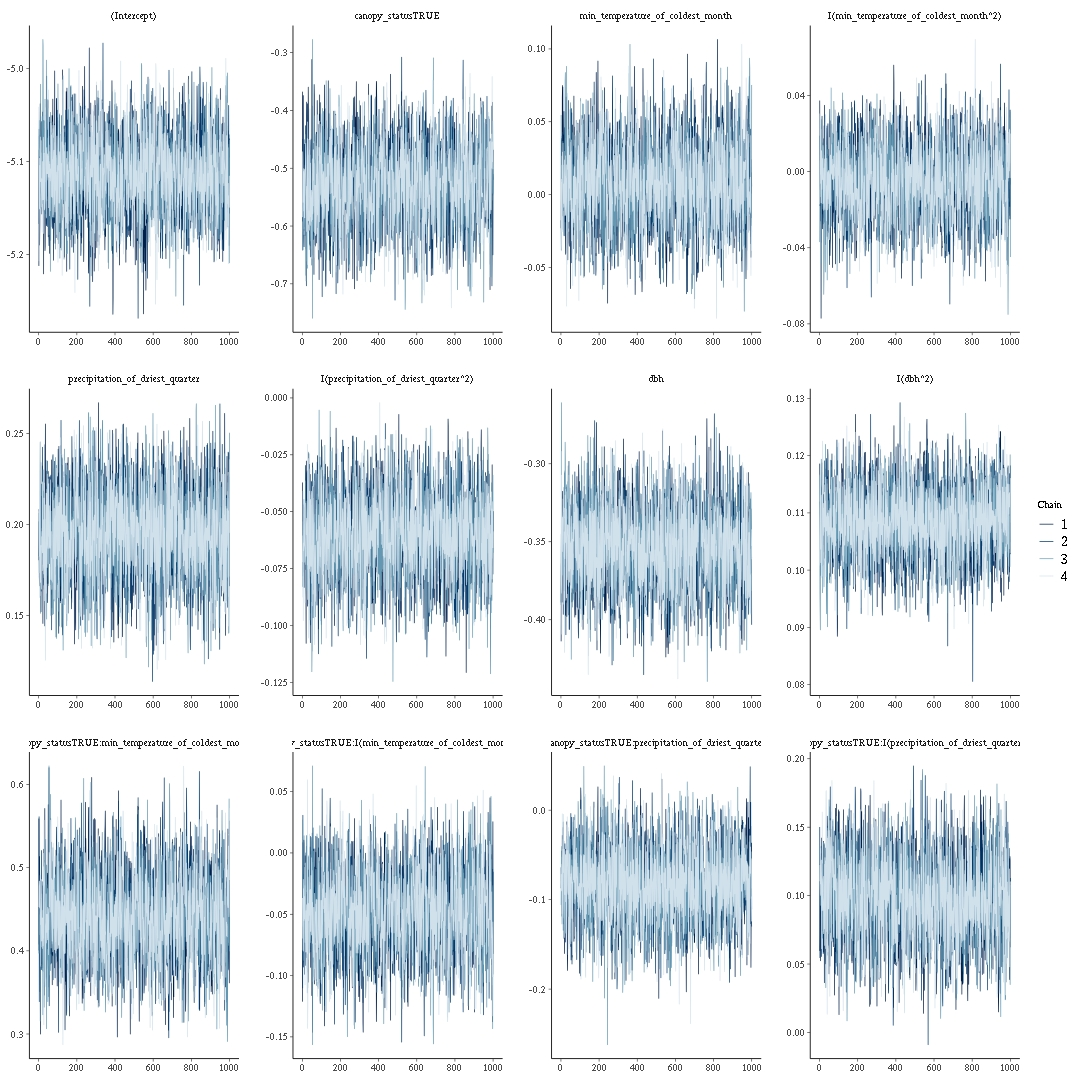
\includegraphics[scale=0.4]{./28731-ACE-SAC_traces}
	\caption{\textit{Acer saccharum}}
\end{figure}

\begin{figure}
	\centering
	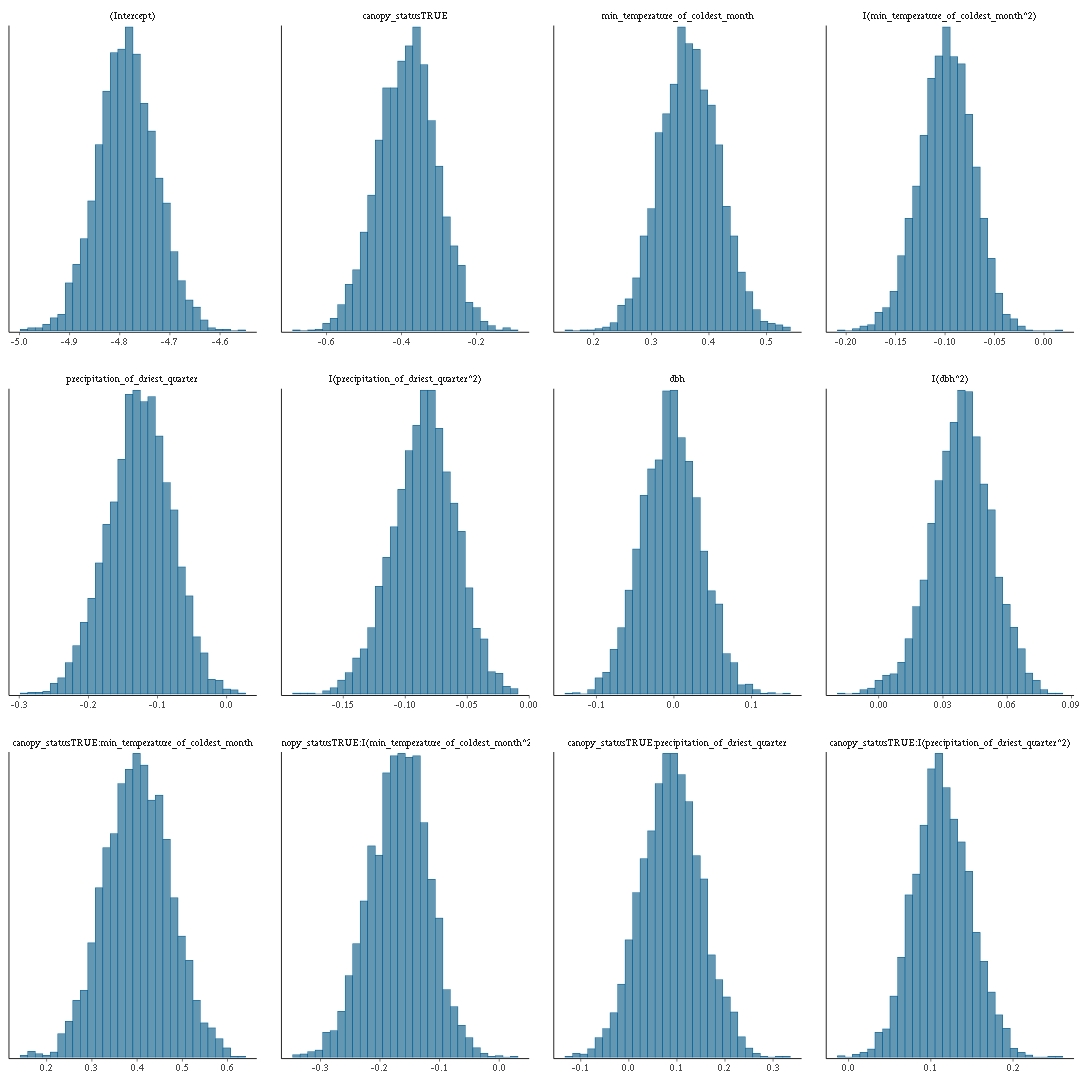
\includegraphics[scale=0.4]{./19481-BET-ALL_hist}
	\caption{\textit{Betula alleghaniensis}}
\end{figure}

\begin{figure}
	\centering
	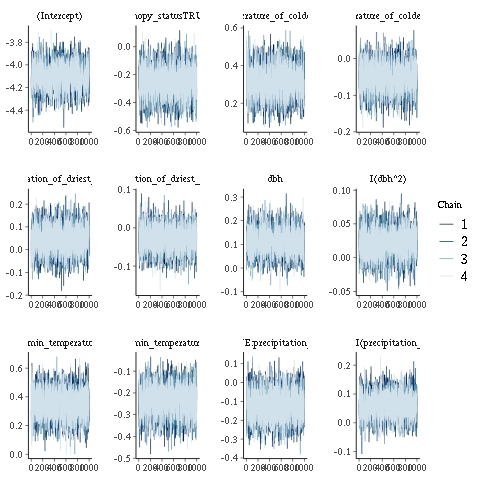
\includegraphics[scale=0.4]{./19481-BET-ALL_traces}
	\caption{\textit{Betula alleghaniensis}}
\end{figure}

\begin{figure}
	\centering
	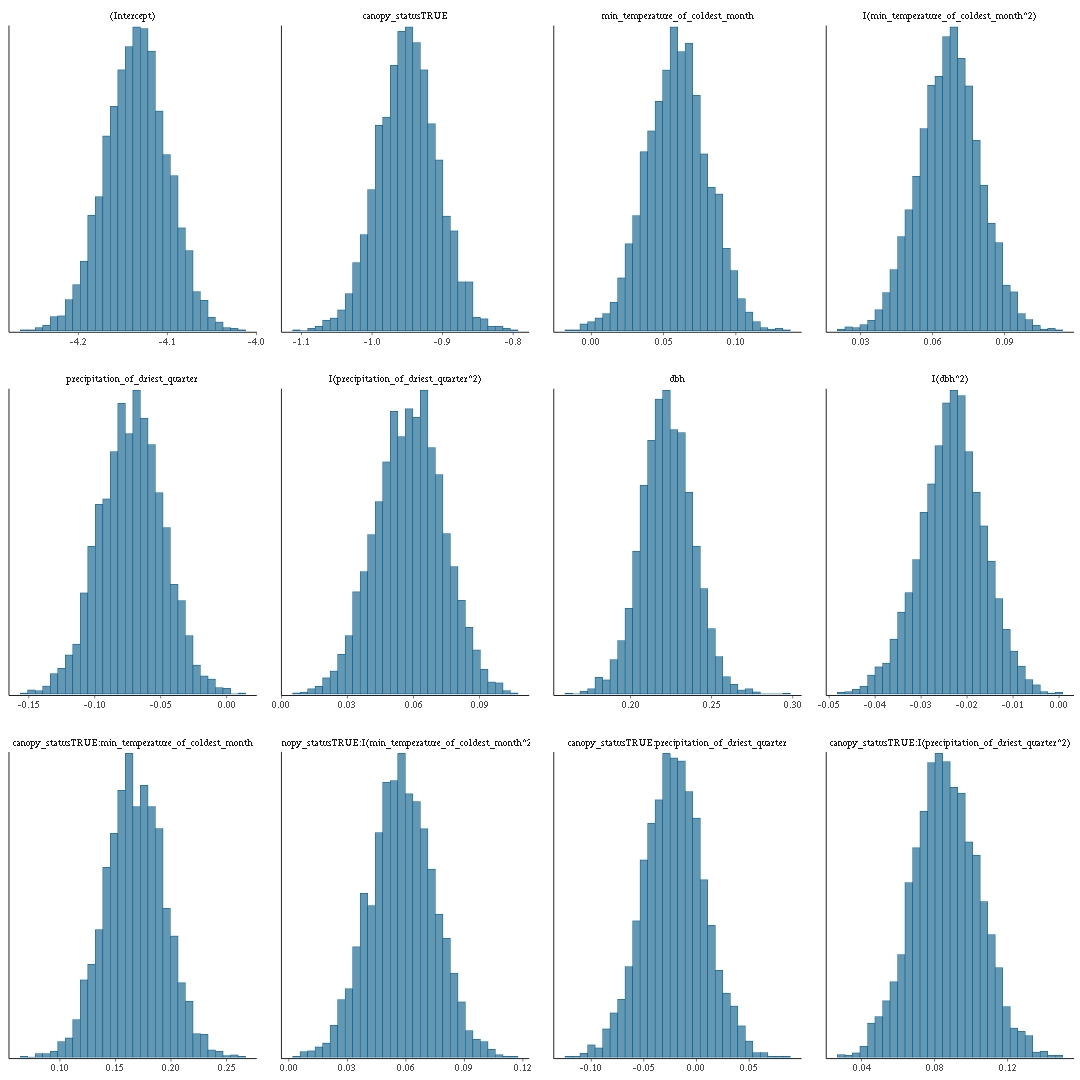
\includegraphics[scale=0.4]{./19489-BET-PAP_hist}
	\caption{\textit{Betula papyrifera}}
\end{figure}

\begin{figure}
	\centering
	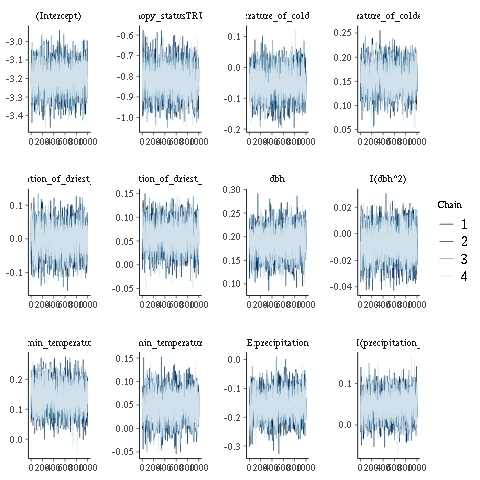
\includegraphics[scale=0.4]{./19489-BET-PAP_traces}
	\caption{\textit{Betula papyrifera}}
\end{figure}

\begin{figure}
	\centering
	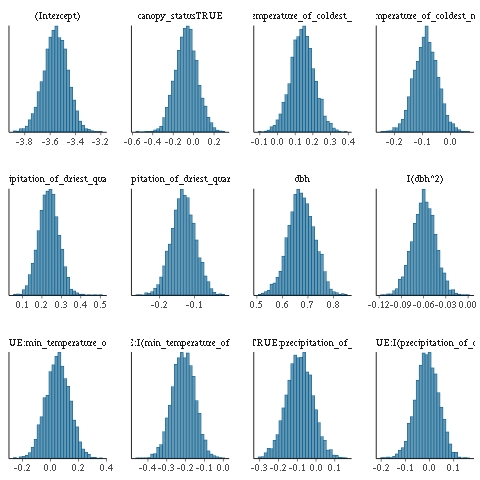
\includegraphics[scale=0.4]{./19462-FAG-GRA_hist}
	\caption{\textit{Fagus grandifolia}}
\end{figure}

\begin{figure}
	\centering
	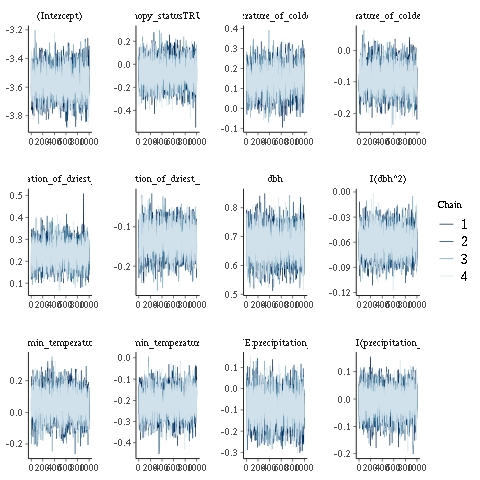
\includegraphics[scale=0.4]{./19462-FAG-GRA_traces}
	\caption{\textit{Fagus grandifolia}}
\end{figure}

\begin{figure}
	\centering
	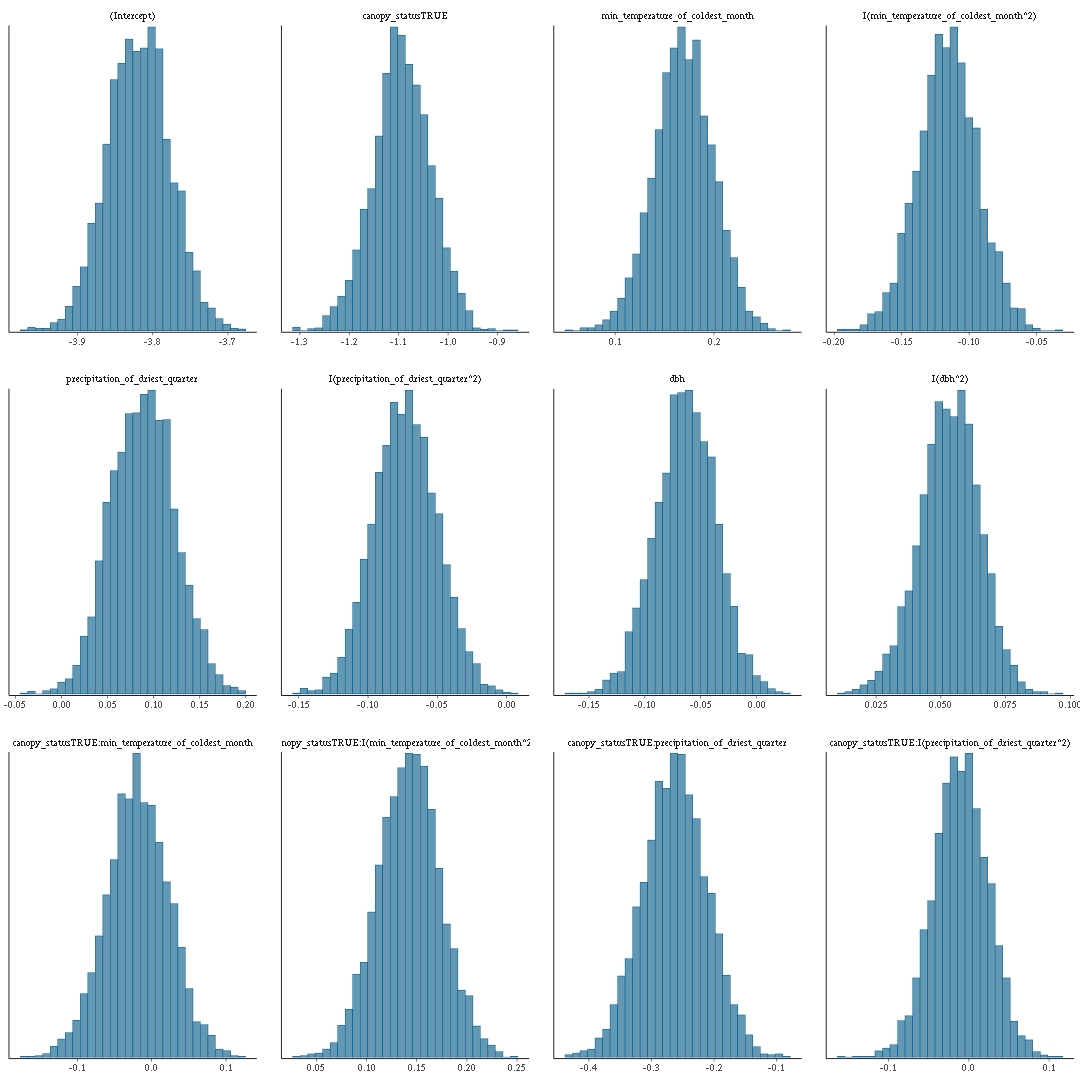
\includegraphics[scale=0.4]{./183295-PIC-GLA_hist}
	\caption{\textit{Picea glauca}}
\end{figure}

\begin{figure}
	\centering
	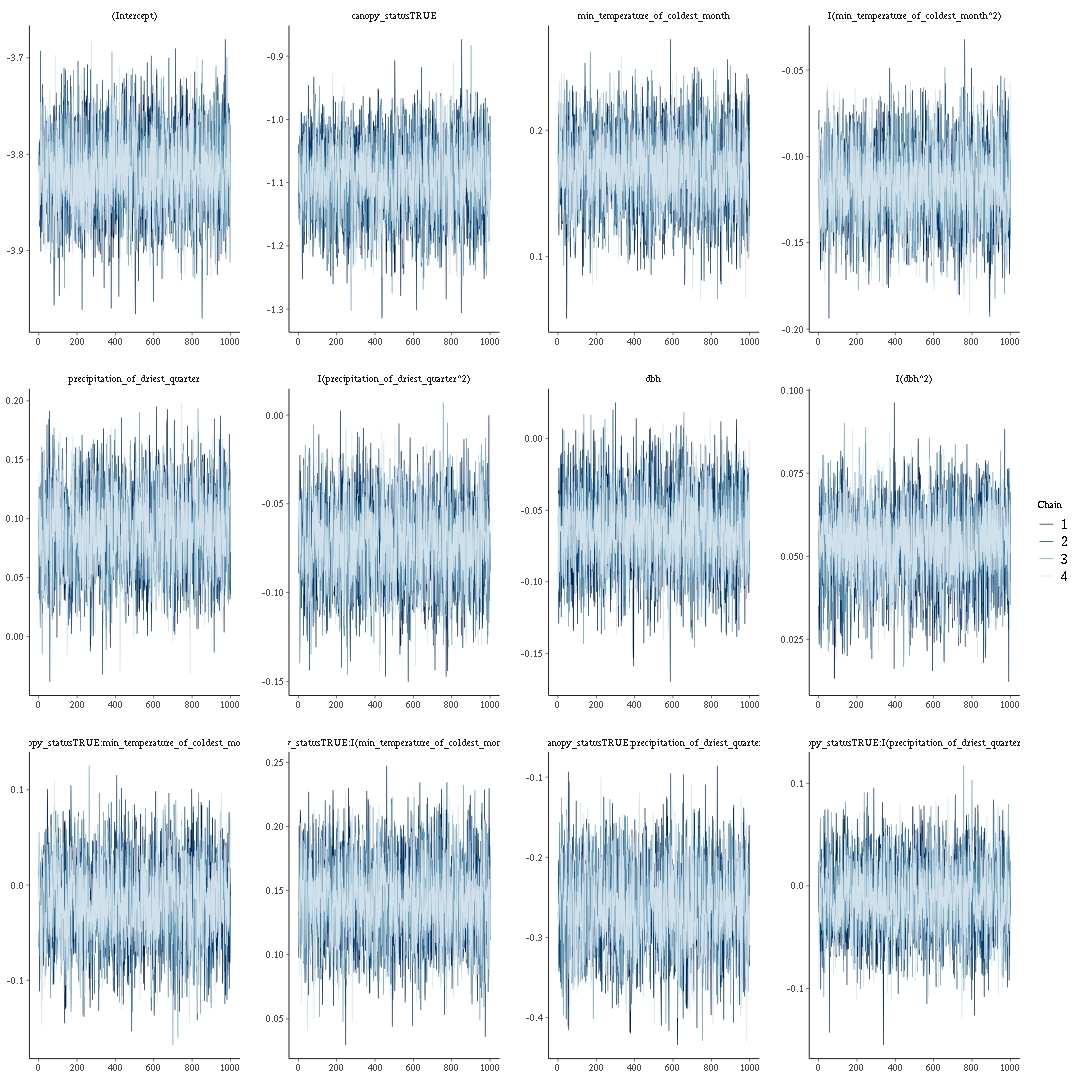
\includegraphics[scale=0.4]{./183295-PIC-GLA_traces}
	\caption{\textit{Picea glauca}}
\end{figure}

\begin{figure}
	\centering
	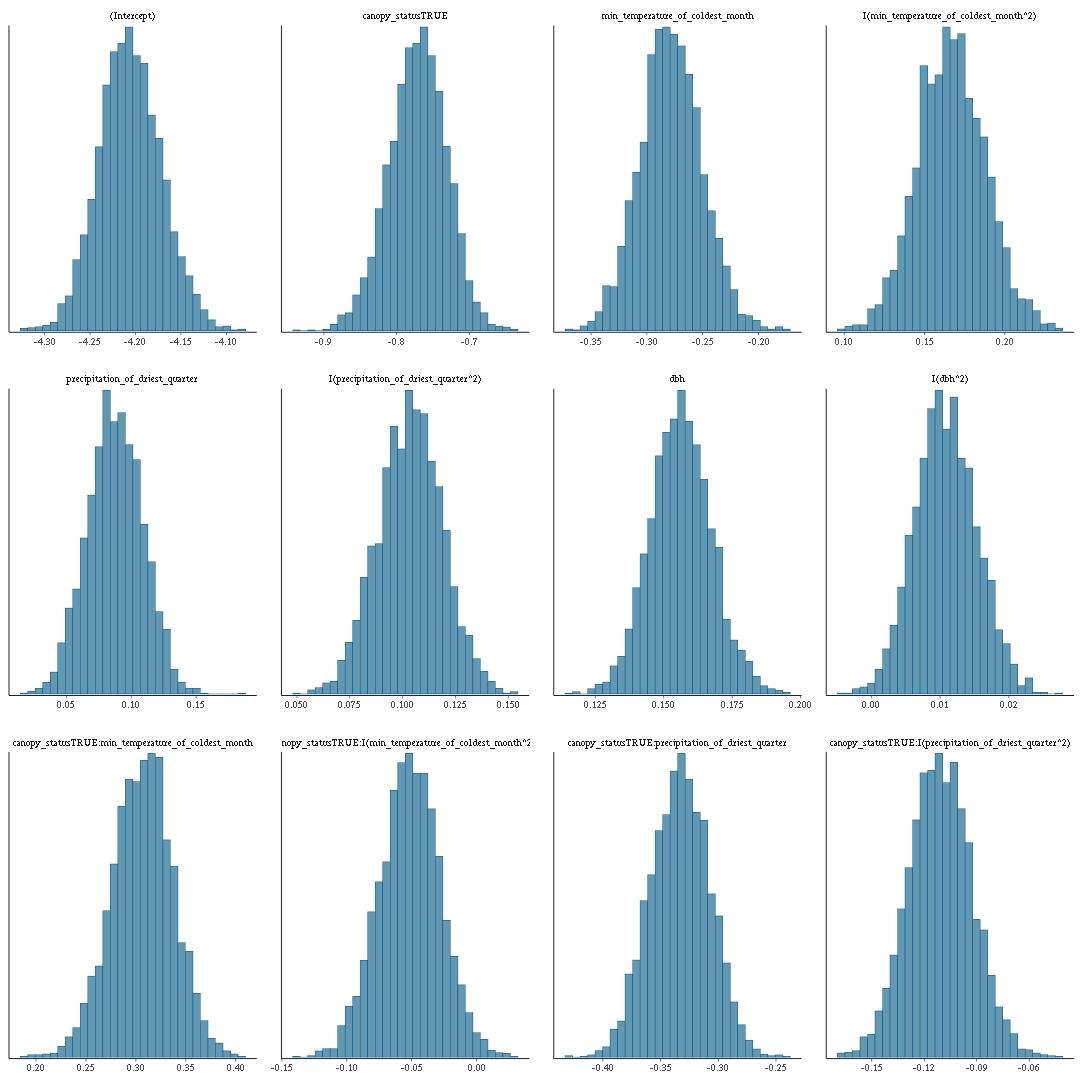
\includegraphics[scale=0.4]{./183302-PIC-MAR_hist}
	\caption{\textit{Picea mariana}}
\end{figure}

\begin{figure}
	\centering
	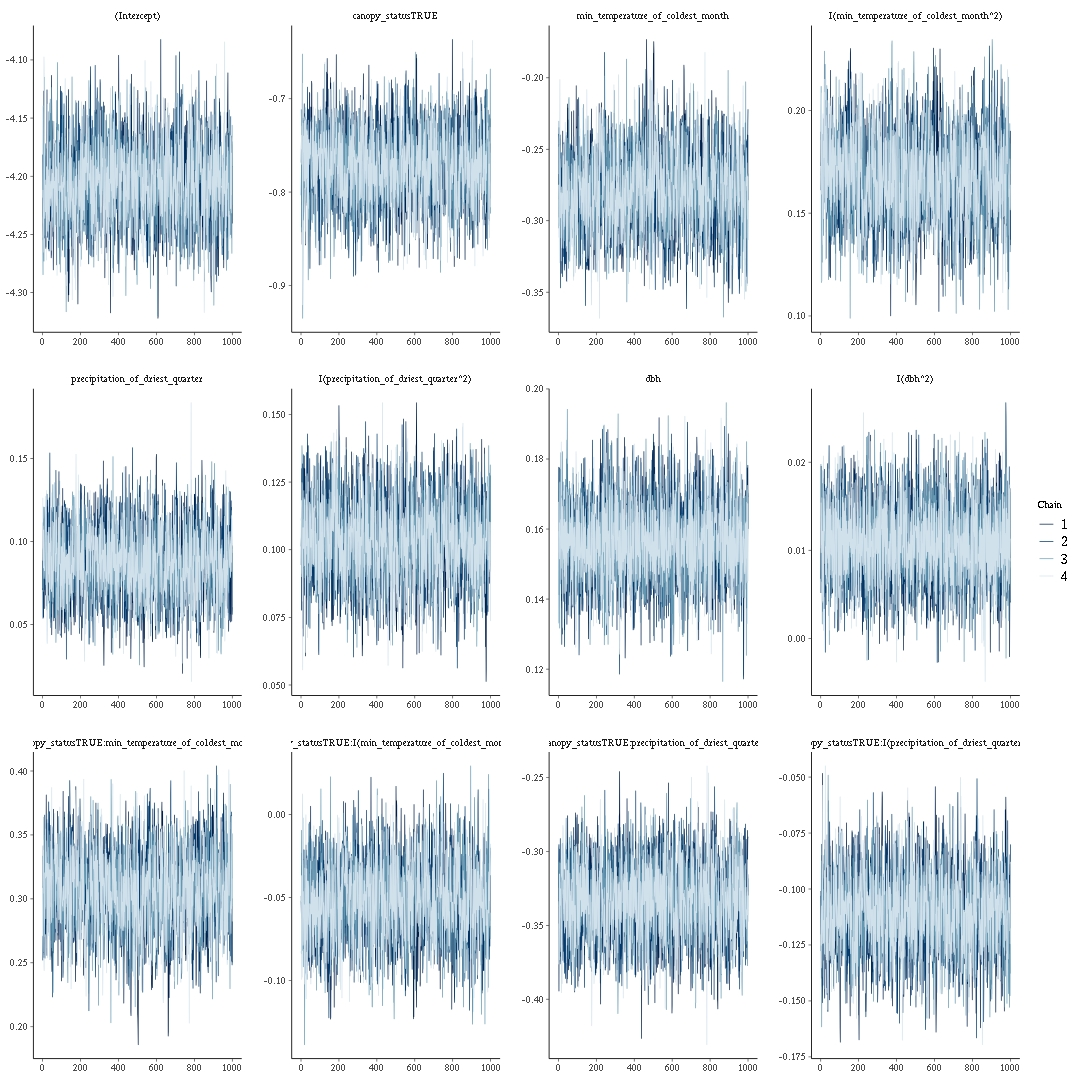
\includegraphics[scale=0.4]{./183302-PIC-MAR_traces}
	\caption{\textit{Picea mariana}}
\end{figure}

\begin{figure}
	\centering
	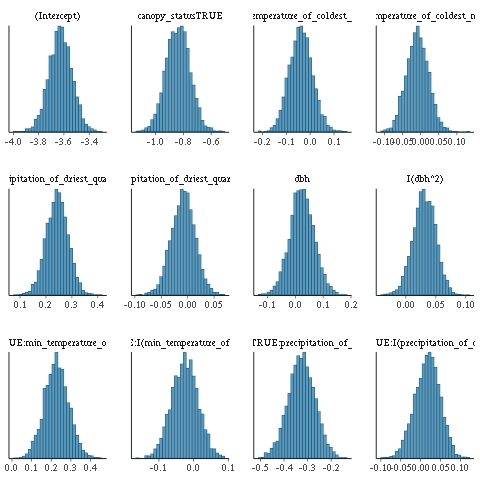
\includegraphics[scale=0.4]{./18034-PIC-RUB_hist}
	\caption{\textit{Picea rubens}}
\end{figure}

\begin{figure}
	\centering
	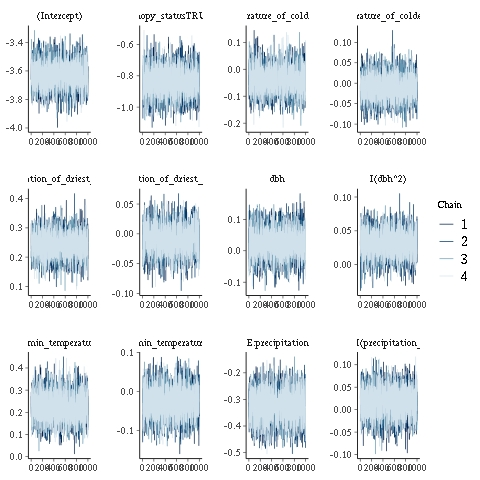
\includegraphics[scale=0.4]{./18034-PIC-RUB_traces}
	\caption{\textit{Picea rubens}}
\end{figure}

\begin{figure}
	\centering
	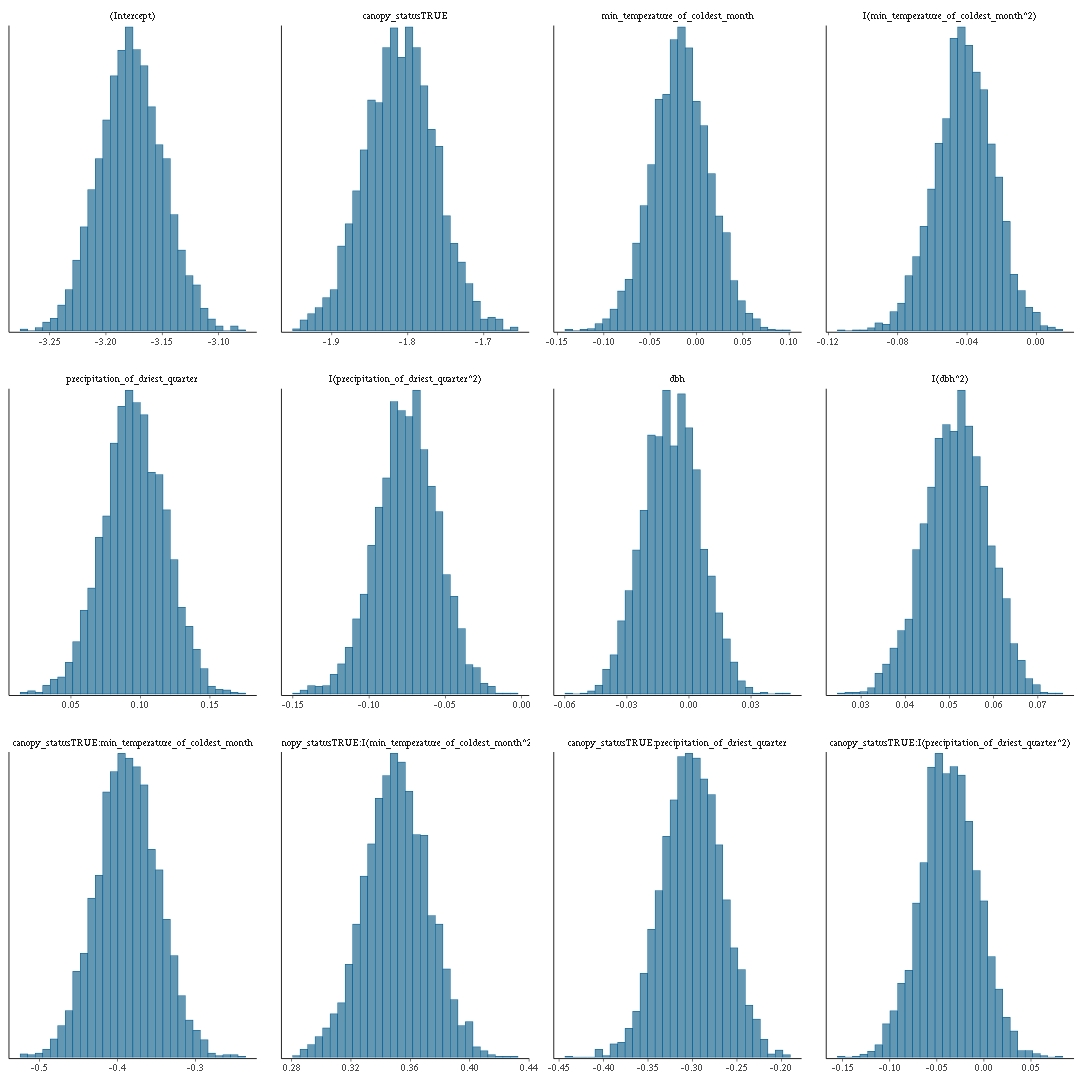
\includegraphics[scale=0.4]{./183319-PIN-BAN_hist}
	\caption{\textit{Pinus banksiana}}
\end{figure}

\begin{figure}
	\centering
	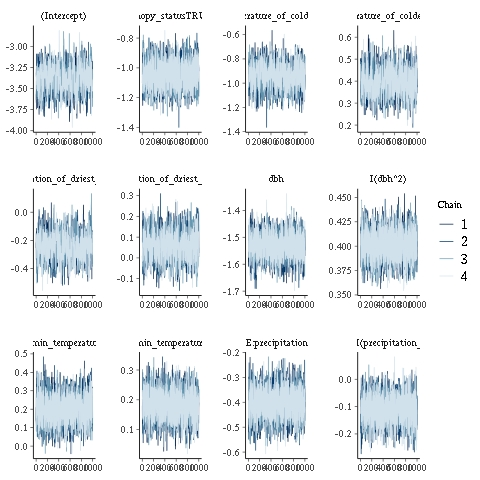
\includegraphics[scale=0.4]{./183319-PIN-BAN_traces}
	\caption{\textit{Pinus banksiana}}
\end{figure}

\begin{figure}
	\centering
	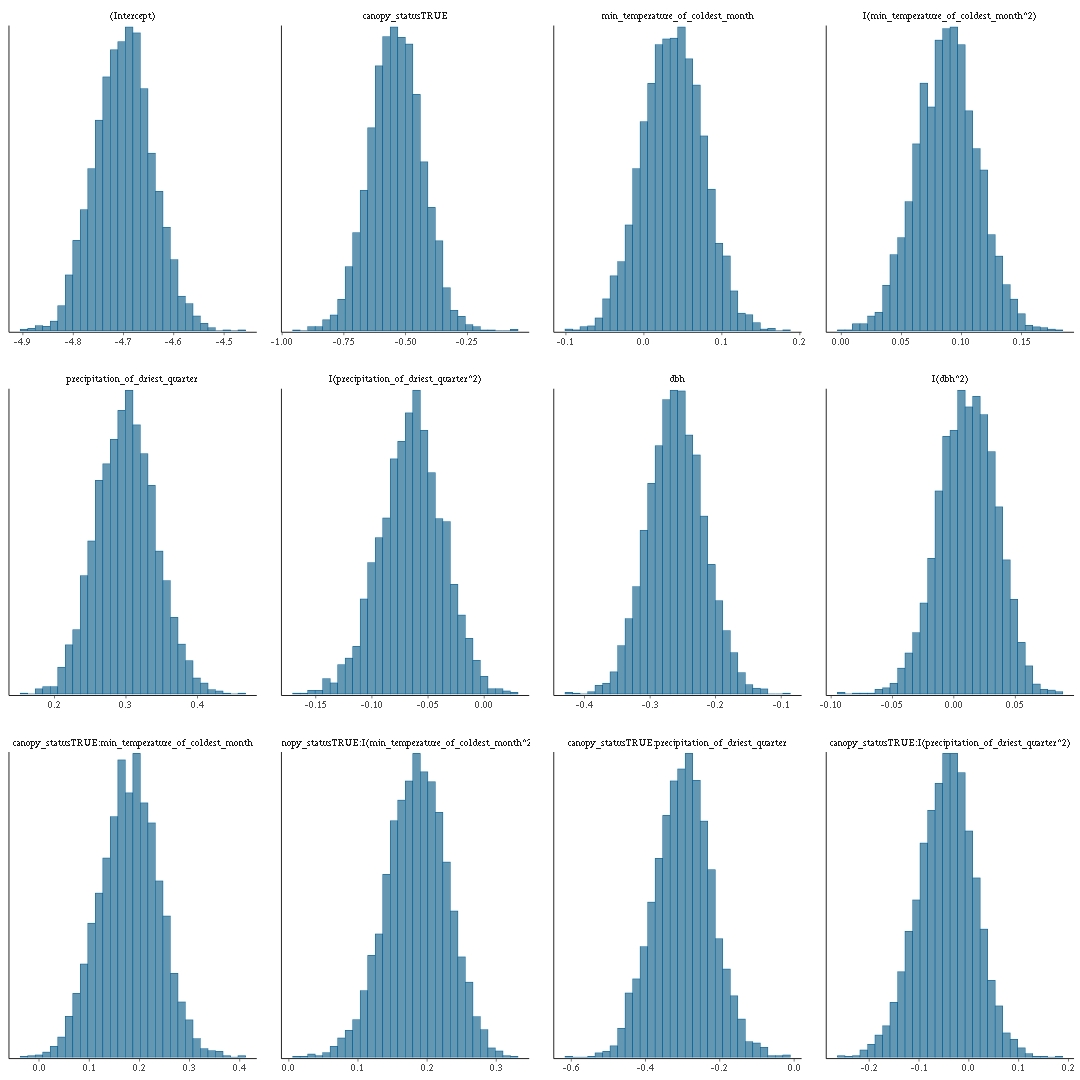
\includegraphics[scale=0.4]{./183385-PIN-STR_hist}
	\caption{\textit{Pinus strobus}}
\end{figure}

\begin{figure}
	\centering
	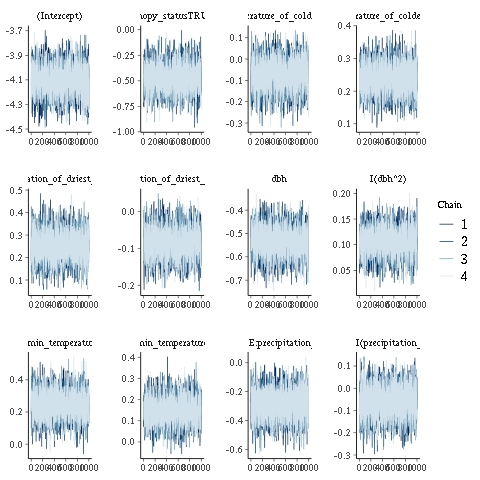
\includegraphics[scale=0.4]{./183385-PIN-STR_traces}
	\caption{\textit{Pinus strobus}}
\end{figure}

\begin{figure}
	\centering
	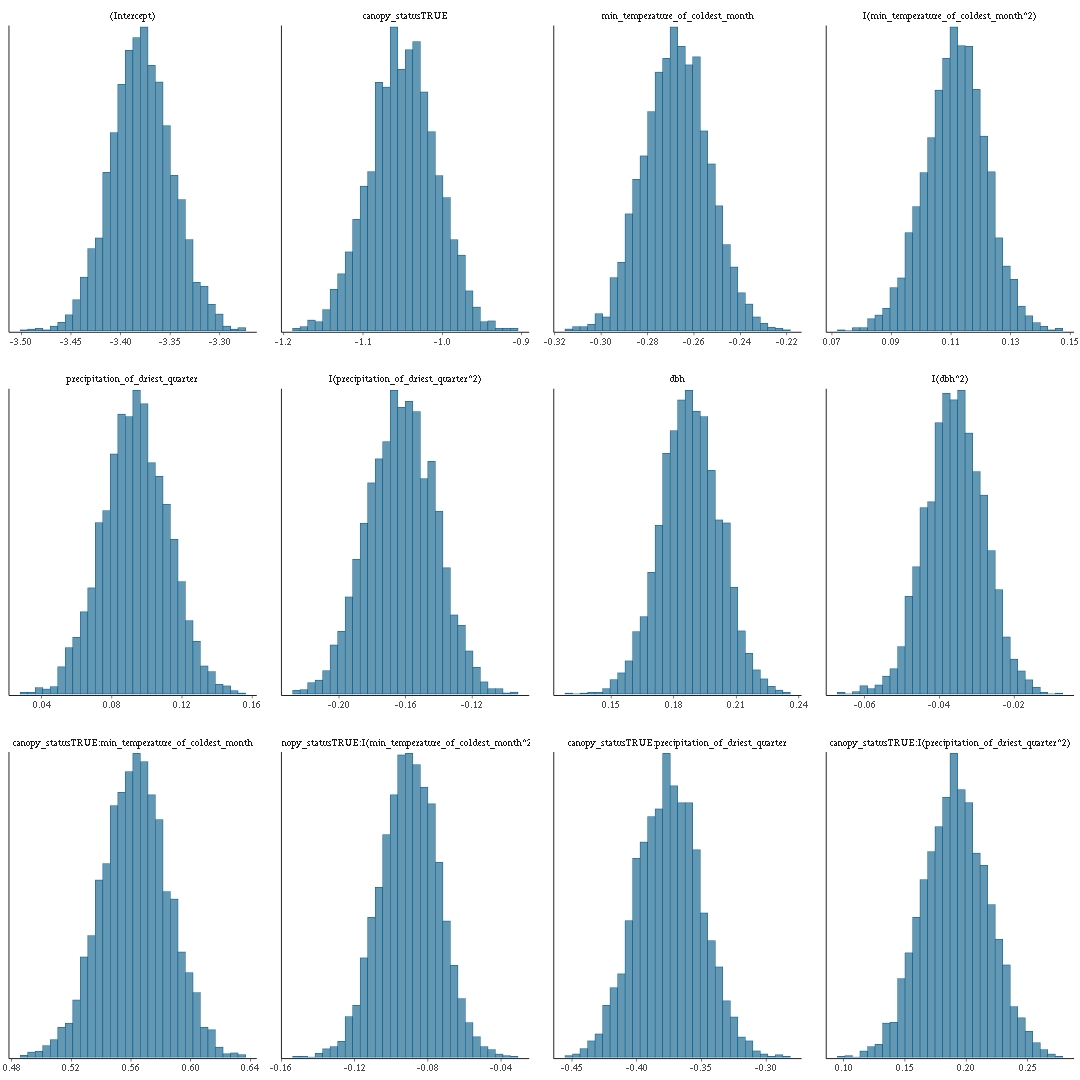
\includegraphics[scale=0.4]{./195773-POP-TRE_hist}
	\caption{\textit{Populus tremuloides}}
\end{figure}

\begin{figure}
	\centering
	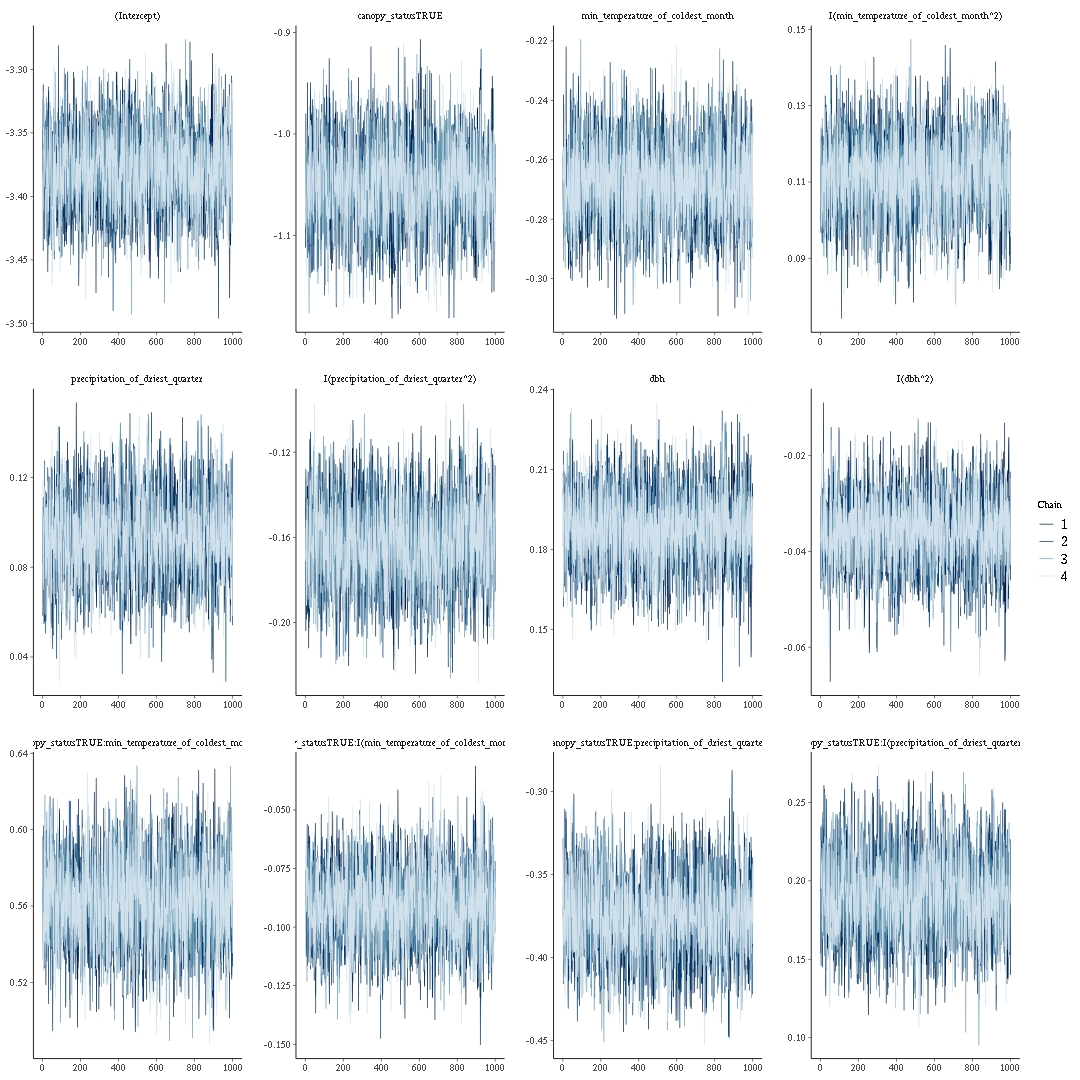
\includegraphics[scale=0.4]{./195773-POP-TRE_traces}
	\caption{\textit{Populus tremuloides}}
\end{figure}

\begin{figure}
	\centering
	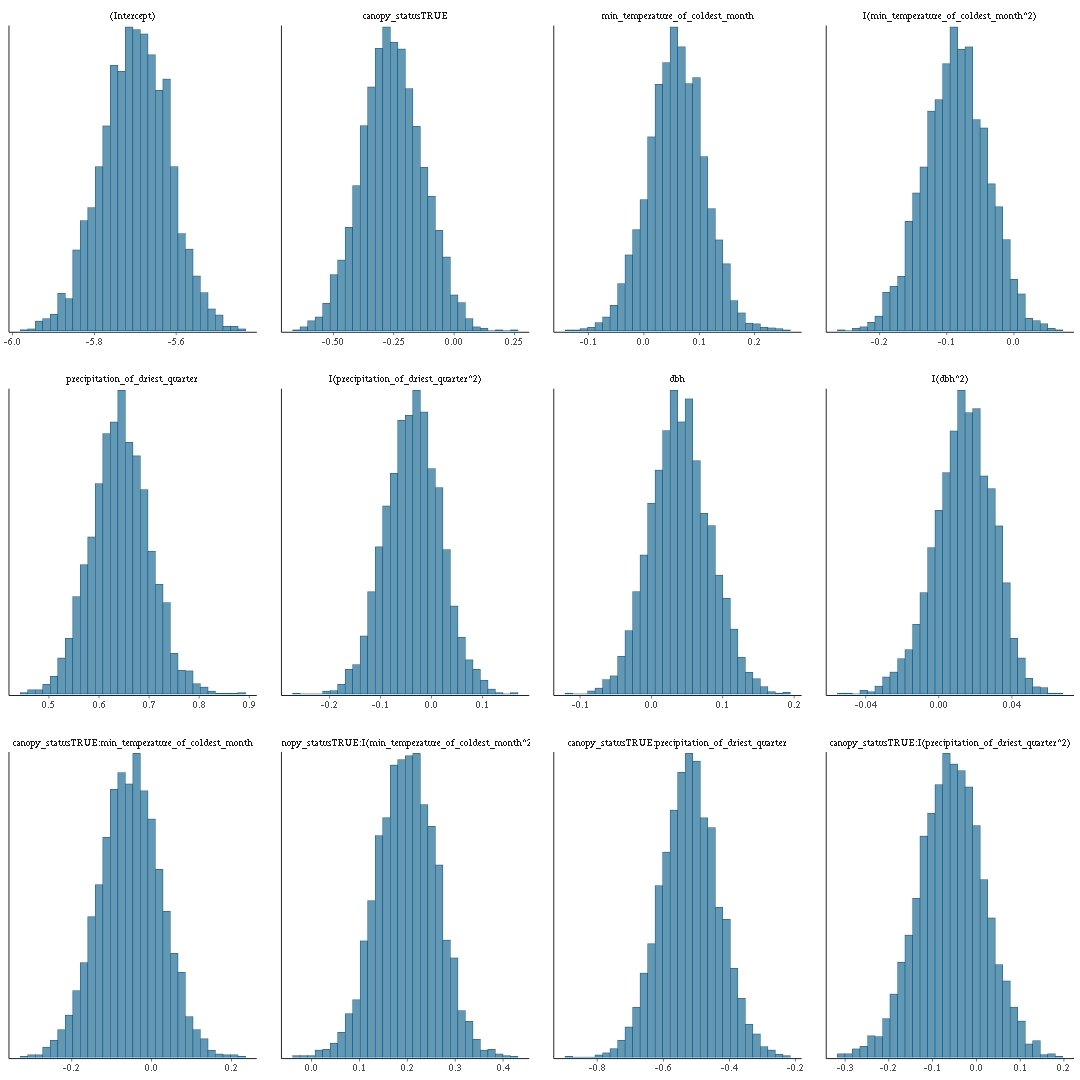
\includegraphics[scale=0.4]{./505490-THU-OCC_hist}
	\caption{\textit{Thuja occidentalis}}
\end{figure}

\begin{figure}
	\centering
	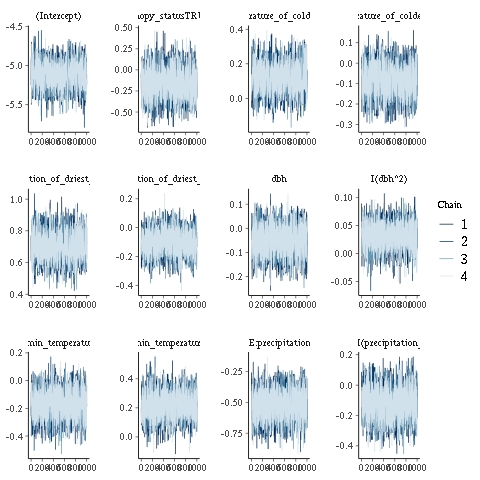
\includegraphics[scale=0.4]{./505490-THU-OCC_traces}
	\caption{\textit{Thuja occidentalis}}
\end{figure}

\begin{figure}
	\centering
	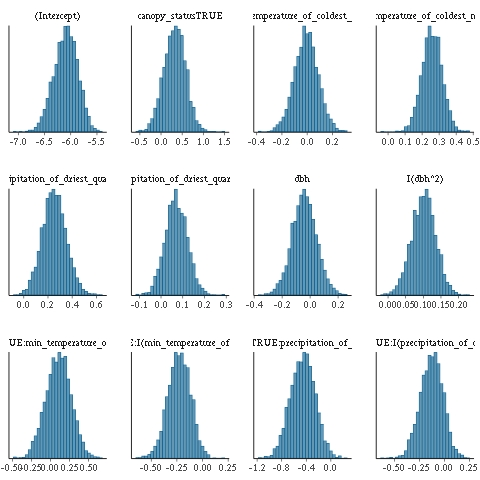
\includegraphics[scale=0.4]{./183397-TSU-CAN_hist}
	\caption{\textit{Tsuga canadensis}}
\end{figure}

\begin{figure}
	\centering
	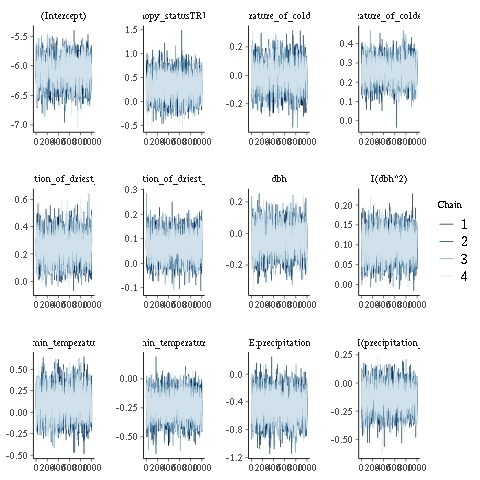
\includegraphics[scale=0.4]{./183397-TSU-CAN_traces}
	\caption{\textit{Tsuga canadensis}}
\end{figure}

\end{document}
